% !TEX root =  ../Main.tex
\subsection{Space Software Mutation Testing Process}
\label{sec:approach}

\begin{figure}[tb]
\begin{center}
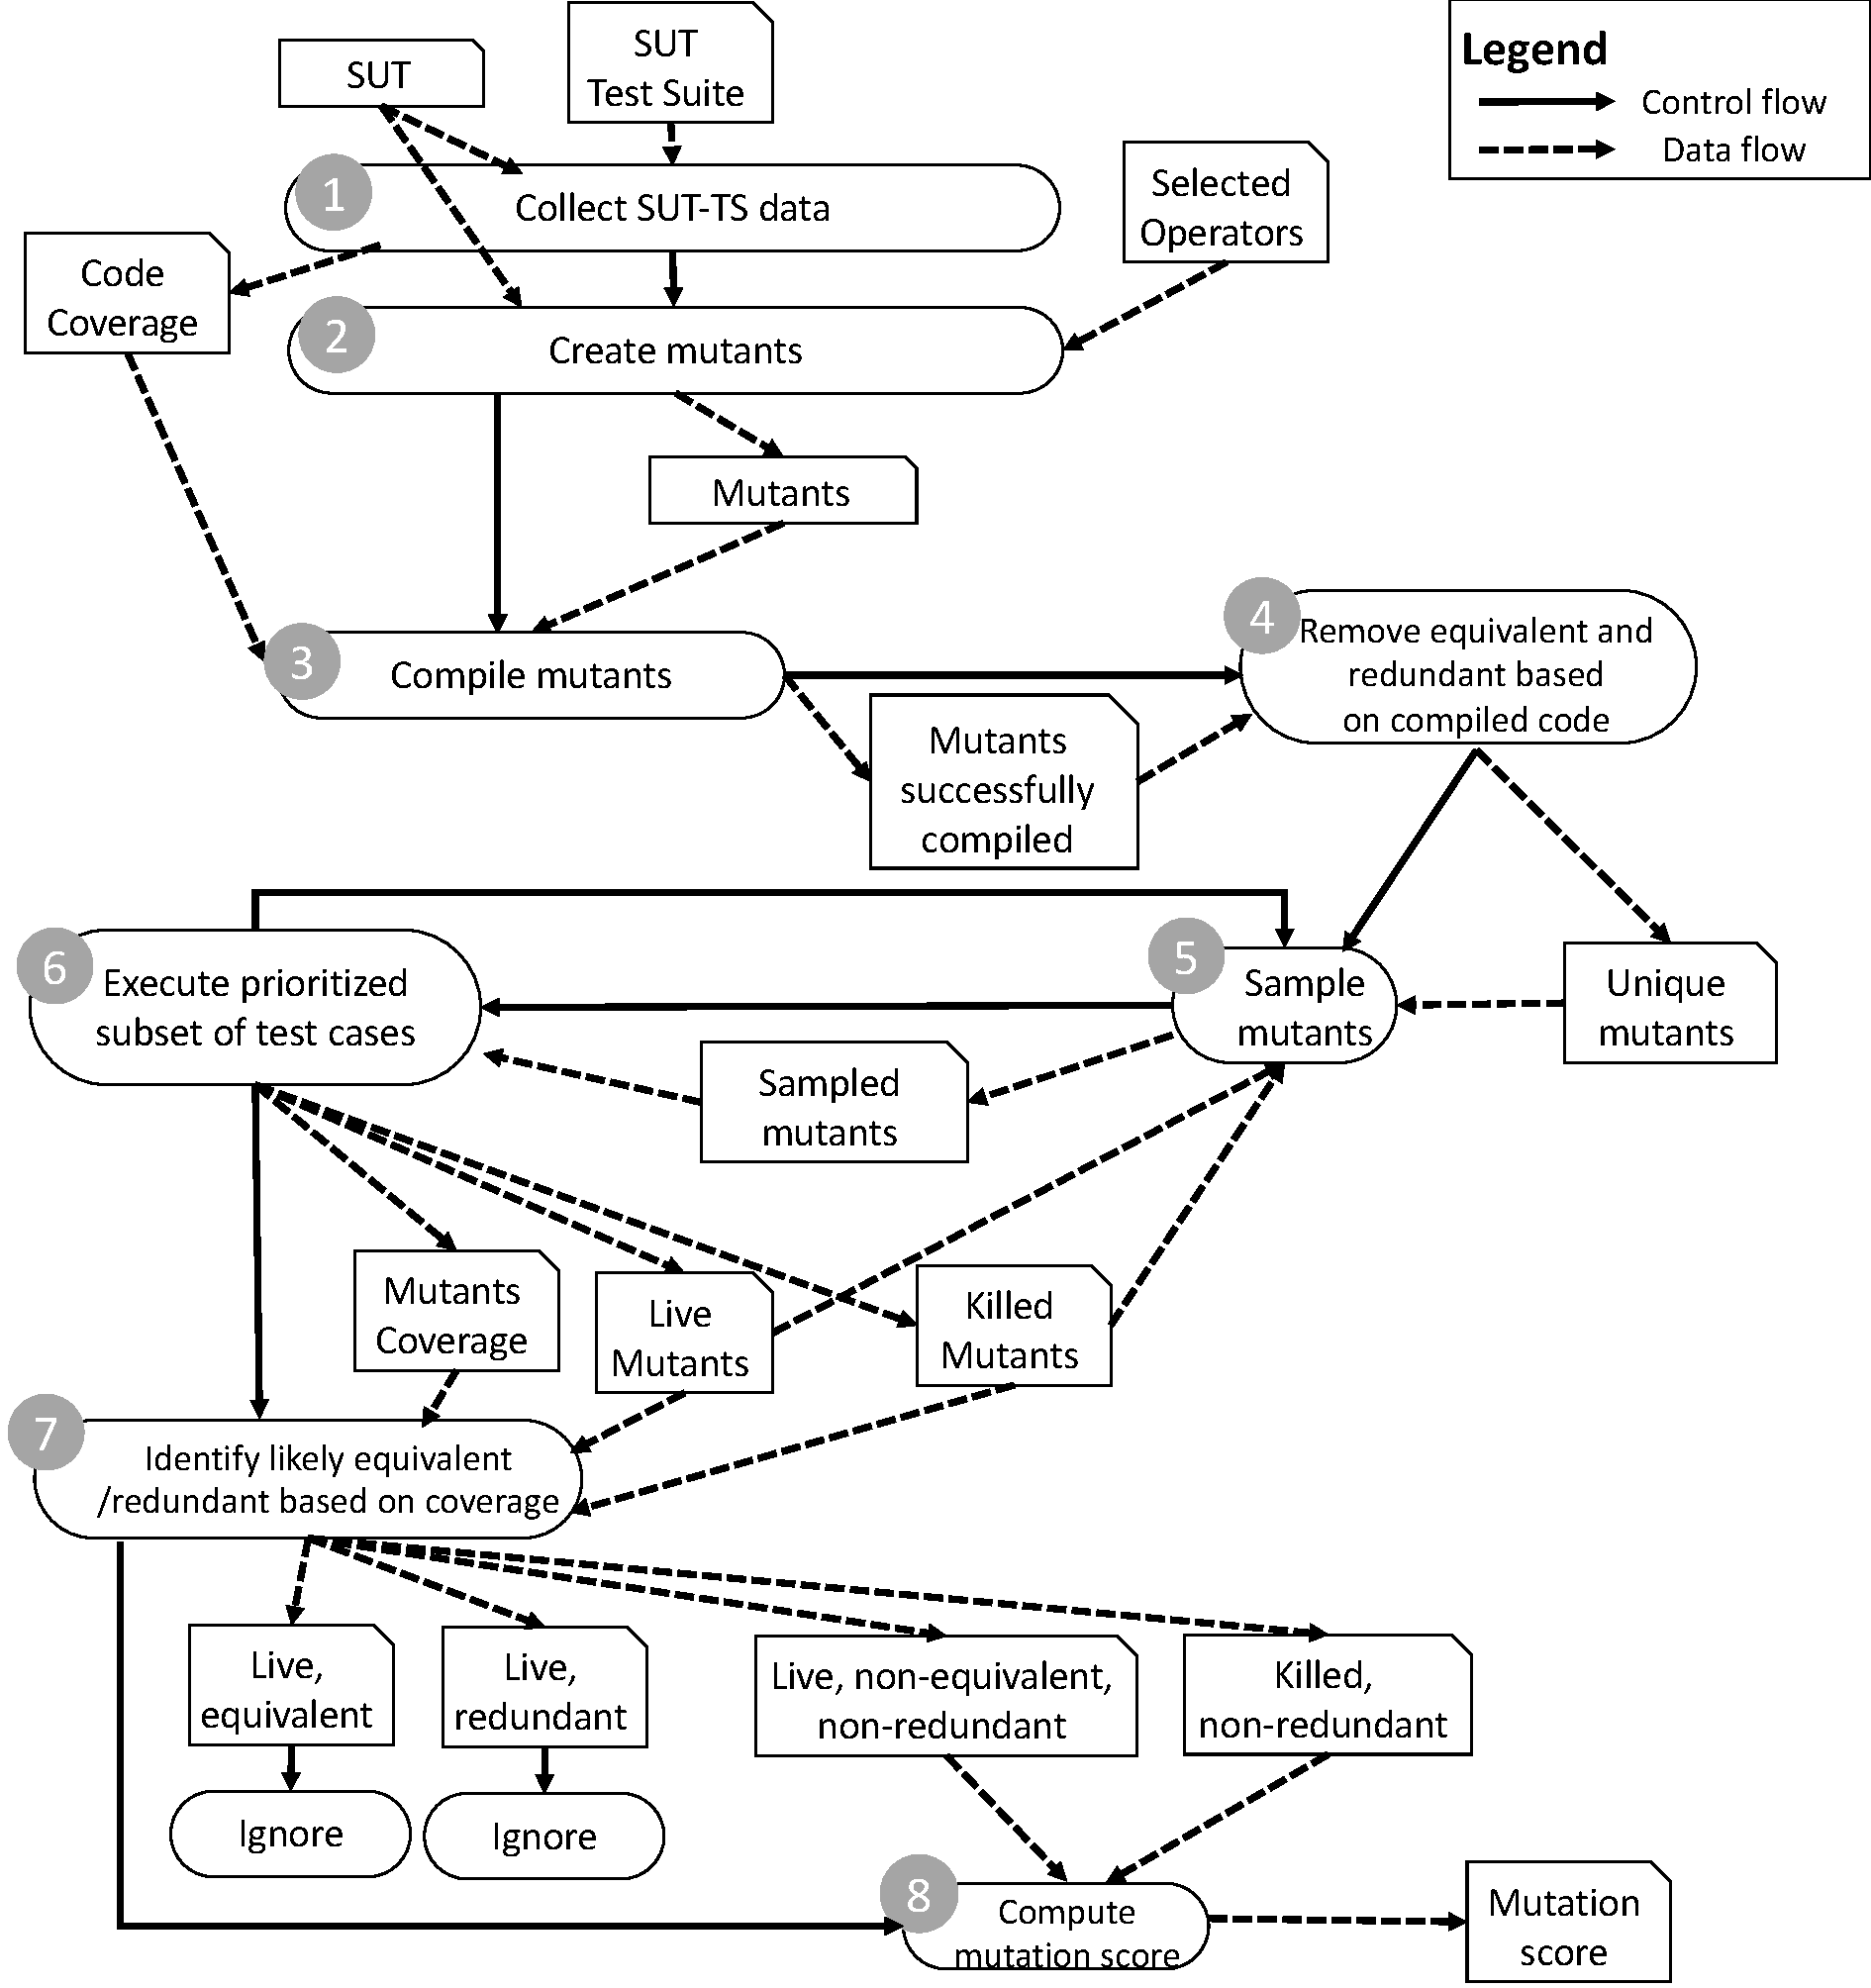
\includegraphics[width=8cm]{images/Approach}
\caption{Overview of the proposed Mutation Testing Pipeline}
\label{fig:approach}
\end{center}
\end{figure}

Figure~\ref{fig:approach} provides an overview of the mutation testing process that we propose, namely Scalable Mutation Testing for Space Software  (\APPR). We describe each step in the following paragraphs. 

\subsubsection{Step 1}

In Step 1, the test suite is executed against the software under test (SUT) and code coverage information is collected. 
More precisely, we rely state-of-the art code coverage tools such as gcov~\cite{GCOV} and Vector CAST~\cite{VectorCAST} 
to record the number of times each line of code of the SUT has been exercised by a test case.

\subsubsection{Step 2}

In Step 2, we automatically generate mutants for the SUT by relying on a set of selected mutation operators.
In \APPR, based on the considerations provided in Section~\ref{sec:related:operators}, we rely on an extended sufficient set of mutation operators, which are listed in Table~\ref{table:sufficient_operators}.
In addition, in our experiments, we evaluate the feasibility of relying only on the SDL operators instead of the whole sufficient set of operators.

% !TEX root =  ../Main.tex

\newcommand{\op}{\mathit{op}}
\newcommand{\ArithmeticSet}{ \texttt{+}, \texttt{-}, \texttt{*}, \texttt{/}, \texttt{\%} }
\newcommand{\LogicalSet}{ \texttt{&&}, \texttt{||} }
\newcommand{\RelationalSet}{ \texttt{>}, \texttt{>=}, \texttt{<}, \texttt{<=}, \texttt{==}, \texttt{!=} }
\newcommand{\BitWiseSet}{ \texttt{\&}, \texttt{|}, \land }
\newcommand{\ShiftSet}{ \texttt{>>}, \texttt{<<} }


\begin{table}[h]
\caption{Implemented set of mutation operators.}
\label{table:operators} 
\centering
\scriptsize
\begin{tabular}{|@{}p{4mm}@{}|@{}p{2cm}@{\hspace{1pt}}|@{}p{11.1cm}@{}|}
\hline
&\textbf{Operator} & \textbf{Description$^{*}$} \\
\hline
\multirow{7}{*}{\rotatebox{90}{\emph{Sufficient Set}}}&ABS               & $\{(v, -v)\}$	\\
\cline{2-3}
&AOR               & $\{(\op_1, op_2) \,|\, \op_1, \op_2 \in \{ \ArithmeticSet \} \land \op_1 \neq \op_2 \} $       \\
&    			  & $\{(\op_1, \op_2) \,|\, \op_1, \op_2 \in \{\texttt{+=}, \texttt{-=}, \texttt{*=}, \texttt{/=}, \texttt{\%} \texttt{=}\} \land \op_1 \neq \op_2 \} $       \\
\cline{2-3}
&ICR               & $\{i, x) \,|\, x \in \{1, -1, 0, i + 1, i - 1, -i\}\}$           \\
\cline{2-3}
&LCR               & $\{(\op_1, \op_2) \,|\, \op_1, \op_2 \in \{ \texttt{\&\&}, || \} \land \op_1 \neq \op_2 \}$            \\
&				  & $\{(\op_1, \op_2) \,|\, \op_1, \op_2 \in \{ \texttt{\&=}, \texttt{|=}, \texttt{\&=}\} \land \op_1 \neq \op_2 \}$            \\
&				  & $\{(\op_1, \op_2) \,|\, \op_1, \op_2 \in \{ \texttt{\&}, \texttt{|}, \texttt{\&\&}\} \land \op_1 \neq \op_2 \}$            \\
\cline{2-3}
&ROR               & $\{(\op_1, \op_2) \,|\, \op_1, \op_2 \in \{ \RelationalSet \}\}$            \\
&				  & $\{ (e, !(e)) \,|\, e \in \{\texttt{if(e)}, \texttt{while(e)}\} \}$ \\
\cline{2-3}
&SDL               & $\{(s, \texttt{remove}(s))\}$            \\
\cline{2-3}
&UOI               & $\{ (v, \texttt{--}v), (v, v\texttt{--}), (v, \texttt{++}v), (v, v\texttt{++}) \}$            \\   
\hline
\hline
\multirow{5}{*}{\rotatebox{90}{\emph{OODL}}}&AOD               & $\{((t_1\,op\,t_2), t_1), ((t_1\,op\,t_2), t_2) \,|\, op \in \{ \ArithmeticSet \} $       \\ 
\cline{2-3}
&LOD               & $\{((t_1\,op\,t_2), t_1), ((t_1\,op\,t_2), t_2) \,|\, op \in \{  \} \}$       \\ 
\cline{2-3}
&ROD               & $\{((t_1\,op\,t_2), t_1), ((t_1\,op\,t_2), t_2) \,|\, op \in \{ \RelationalSet \} \}$       \\ 
\cline{2-3}
&BOD               & $\{((t_1\,op\,t_2), t_1), ((t_1\,op\,t_2), t_2) \,|\, op \in \{ \BitWiseSet \} \}$       \\ 
\cline{2-3}
&SOD               & $\{((t_1\,op\,t_2), t_1), ((t_1\,op\,t_2), t_2) \,|\, op \in \{ \ShiftSet \} \}$       \\ 
%\hline
%COR               & $\{(\op_1, \op_2) \,|\, \op_1, \op_2 \in \{ \texttt{\&\&}, \texttt{||}, \land \} \land \op_1 \neq \op_2 \}$            \\
\hline
\hline
\multirow{3}{*}{\rotatebox{90}{\emph{Other}}}&LVR			& $\{(l_1, l_2) \,|\, (l_1, l_2) \in \{(0,-1), (l_1,-l_1), (l_1, 0), (\mathit{true}, \mathit{false}), (\mathit{false}, \mathit{true})\}\}$\\
&&\\
&&\\
\hline
\end{tabular}

$^{*}$Each pair in parenthesis shows how a program element is modified by the mutation operator. Th eleft element of the pair is replaced with the right element. We follow standard syntax~\cite{kintis2018effective}. Program elements are literals ($l$), integer literals ($i$), boolean expressions ($e$), operators ($\op$), statements ($s$), variables ($v$), and terms ( $t_i$, which might be either variables or literals).
\end{table}

To automatically generate mutants, we have extended SRCIRor~\cite{hariri2018srciror} to include all the mutation operators of the sufficient set. After mutating the original source file, our extension saves the mutated source file and keeps track of the mutation applied. 

\subsubsection{Step 3}

In Step 3, we compile mutants by relying on the build system of the SUT. To this end, we have developed a toolset that, for each mutated source file: (1) backs-up the original source file, (2) renames the mutated source file as the original source file, (3) runs the build system (e.g., executes the command \texttt{make}), (4) copies the generated executable mutant in a dedicated folder, (5) restores the original source file. 

Build systems create one object file for each source file to be compiled and then link these object files together into the final executable. For this reason, since we modify at most two source files for each mutant (i.e., the mutated file and the file restored from previous mutation), we can reuse almost all the compiled object files in subsequent compilation runs, thus speeding up the compilation of multiple mutants. Some preliminary experiments conducted with our case study systems have shown that additional compile-time optimizations (e.g., mutant schemata) are not necessary to make the compilation of mutants feasible.

\subsubsection{Step 4}

In Step 4, we rely on trivial compiler optimizations to identify and remove equivalent and redundant mutants. 
\MREVISION{C-P-15}{We aim to enable all the available optimizations (e.g., \texttt{-O3} or \texttt{-Ofast} in GCC).}
If the SUT is already configured to be compiled with optimizations enabled, Step 4 consists of first computing the SHA-512 hash summary of all the mutant and original executables and then compare all the generated hash summaries. Hash comparison enables us to (1) determine the presence of equivalent mutants (i.e., mutants having the same hash of the original executable), and (2) identify duplicate mutants (i.e., mutants with the same hash). %Mutants that are identified as being either equivalent and redundant mutants are ignored in the following steps of \APPR. 
Equivalent and redundant mutants are discarded.
The outcome of Step 4 is a set of \emph{unique mutants}, i.e., mutants with compiled code that differs from the original software and any other mutant.

If the SUT should not be compiled with compiler optimizations enabled, we identify equivalent and redundant mutants by re-executing Step 3 with compiler optimizations enabled and then apply Step 4.
%The executables generated by this additional run of Step 3 are used only to identify equivalent mutants, not to evaluate the SUT test suite, which is based on executables compiled without optimizations (otherwise test cases may fail).

\subsubsection{Step 5}

In Step 5, we sample the mutants to be executed to compute the mutation score. This optimization is based on the results of Zhang et al.~\cite{zhang2013operator}, who compare eight strategies for sampling mutants. In our work, we consider two strategies. The first is the \emph{baseline sampling} strategy, which consists of randomly selecting $r\%$ mutants from the complete mutants set. The second is the \emph{method-based sampling} strategy, which is the best performing strategy in \cite{zhang2013operator} and consists of sampling mutants evenly across all functions of the SUT, i.e., sampling $r\%$ mutants from each set of mutants generated inside a same function.

%In Section~\ref{}, we evaluate which of these sampling strategies lead to mutation score


\subsubsection{Step 6}

In Step 6, we execute a prioritized subset of test cases. 
We execute test cases in sequence, and we select only the ones that satisfy 
the reachability condition (i.e., cover the mutated statement).
Similarly to the approach of Zhang et al. \cite{zhang2013faster}, we define the order of execution of test cases based on their likelihood of killing a mutant. However, we redefined the criteria for the selection of test cases because of the inapplicability of the ones proposed by Zhang et al. (see Section~\ref{sec:scalability}).

%However, we notice that such optimization may not be sufficient when test suites are particularly large; indeed, prioritizing test cases may not be sufficient to reduce execution time. For example, live mutants may lead to the execution of a large number of test cases when almost all the test cases of the test suite exercise the mutated statement. 


To reduce the number of test cases to be executed with a mutant, 
we should first execute the ones that more likely satisfy the necessity condition. 
More precisely, the next test case to be executed in a sequence should be the one that exercises the mutated statement with variable values not observed before. 
Unfortunately, in our context, the size of the SUT and its real-time constraints prevent us from recording all the variable values processed during testing. 

To determine if two test case executions exercise the mutated statement with diverse variable values, we rely on code coverage.
% as a surrogate indicator of  variable values diversity.
%diversity in values assigned to the variables used in a statement. 
Indeed, a difference in the set of instructions being covered by two test cases that exercise the mutated statement may depend on the values used in the mutated statement. 
However, since the behaviour of the whole software depends on all the executed software instructions, we reduce the scope of our code coverage analysis 
%to the file containing the source code of the mutated function. 
to the mutated function, its callers, and its callees.
%to maximize the chances that a change in the behaviour of the software depends on the values used in a mutated statement, we determine that two executions likely exercise a mutated statement with diverse values by focussing on the coverage of 
%the mutated function, its callers, and its callees.
A reduced scope is effective in determining behavioural differences based on the analysis of variable valuations~\cite{Pastore:VART:2014}.

%Since related work focuses on either statement coverage or the frequency of execution of a statement, 
Following related work, we have identified two possible criteria to characterize test case executions based on code coverage:
\begin{itemize}
\item[C1] Identify the set $C_t$ of source code statements being covered by the test case.
%\item[C2] Identify the set of unique pairs $\langle\mathit{statement},\mathit{arity}\rangle$, where $\mathit{statement}$ is a unique identifier for the source code statement, and $\mathit{arity}$ is a symbol (i.e., $1$ or $*$) indicating if the statement has been covered one or more times.
\item[C2] Derive a vector whose values capture the number of times each monitored statement had been covered.
\end{itemize}

We have identified distance metrics that determine how dissimilar two test cases are, and, consequently how likely they exercise the mutated statement with different values. In the case of C1 we rely on the Jaccard and Ochiai index, which are two similarity indexes for binary data successfully used to compare program executions based on code coverage~\cite{Zou:Ochiai:2019,Keller:Jaccard:2017,Briand:2019}. Given two test cases $T_A$ and $T_B$, the Jaccard  ($D_J$) and the Ochiai ($D_O$) distance are computed as follows:

$D_J(T_a,T_b)=\frac{|C_a \cap C_b|}{|C_a \cup C_b|}$ \hspace{5mm} $D_O(T_a,T_b)=1-\frac{|C_a \cap C_b|}{\sqrt{|C_a| * |C_b|}}$, 
$C_a$ and $C_b$ are the set of coverage items exercised by the test cases $T_a$ and $T_b$, respectively.

In the case of C2, we compute the distance between two test cases by relying on the euclidean distance ($D_E$) and the cosine similarity distance ($D_C$), two popular distance metrics used in machine learning. Given two vectors $V_A$ and $V_B$ that capture the number of times each statement has been covered by test cases $T_A$ and $T_B$, the distances $D_E$ and $D_C$ can be computed as follows:

$D_E=\sqrt{\sum_{i=1}^{n}(A_i-B_i)^2}$ 
$D_C= \frac{\sum_{i=1}^{n}A_i*B_i}{\sqrt{\sum_{i=1}^{n}{A_i}^2}*\sqrt{\sum_{i=1}^{n}{B_i}^2}}$,
%Their main difference is that cosine similarity is used when the magnitude of the vectors should not matter.
$A_i$ and $B_i$ refer to the number of times the i-th statement had been covered by test cases $T_A$ and $T_B$, respectively.

Figure~\ref{alg:prioritize} shows the pseudocode of our algorithm for selecting and prioritizing test cases. It generates as output
a prioritized test suite (i.e., \emph{PTS}) that consists of a subset of the test cases that exercise the mutated statement (Line~\ref{alg:prioritize:select}).
Based on the findings of Zhang et al. \cite{zhang2013faster}, we first select the test case that exercises the mutated statement more times (Line~\ref{alg:prioritize:first}) \MREVISION{C-P-17}{ and add it to the prioritized test suite (Line~\ref{alg:prioritize:add}).}
Then, the next selected test case is the one with the largest distance from the closest test case belonging to the set of test cases already selected (Lines~\ref{alg:prioritize:selectStart} to~\ref{alg:prioritize:selectEnd}). 
%is most different than any other test case already included in the prioritized test suite.

%Then, since we aim to maximize test cases diversity, the next selected test case should be the one that is most different than any other test case already included in the prioritized test suite.
%For this reason, for each test case $n$ not selected yet (Line~\ref{alg:prioritize:notSel}), we identify the test case $t$ showing the most similar coverage (i.e., the one with the minimal distance $d$, Line~\ref{alg:prioritize:minD}). We then select the test case $n$ with the highest distance from its closest test case (Lines~\ref{alg:prioritize:selectStart} to~\ref{alg:prioritize:selectEnd}). 

The algorithm iterates as long as it identifies a test case that exercises 
the program instructions differently than the test cases already selected (Line~\ref{alg:prioritize:until}).

Test cases are then executed in the selected order. During the execution we collect code coverage information and identify killed and live mutants.

% !TEX root =  ../Main.tex

\newcommand{\INDA}{10}
\newcommand{\INDB}{15}
\newcommand{\INDC}{5}

%\vspace{-3mm}
\begin{figure}[tb]

\begin{algorithmic}[1]

%\footnotesize
\scriptsize
\Require \emph{TS}, the test suite of the software under test
\Require \emph{Cov}, coverage information, for each test case
\Require \emph{ms}, the mutated statement
\Ensure \emph{PTS}, a list of test cases to be executed, sorted by priority
% (source inputs, follow-up inputs, output data).

\State $\mathit{TS}_m \gets$ subset of $\mathit{TS}$ that cover the mutated statement $\mathit{ms}$, based on \emph{Cov} \label{alg:prioritize:select}
\State $\mathit{PTS} \gets \mathit{new} \mathit{list}$ \textcolor{darkgray}{//this list is initially empty}
\State $\mathit{PTS} \gets$ based on \emph{Cov} select from $\mathit{TS_m}$ the test case $t$ that exercises $\mathit{ms}$ more times \label{alg:prioritize:first}
\State $\mathit{PTS} \gets \mathit{PTS} \cup t$ \textcolor{darkgray}{//include first the test case selected above}  \label{alg:prioritize:add}

\State \textbf{repeat} \label{alg:prioritize:repeat}
\State \hspace{\INDC mm} \textbf{for each} $n$ in the set ($\mathit{TS}_m$ - $\mathit{PTS}$) \textcolor{darkgray}{, which is the set of test cases not already added to $\mathit{PTS}$} \label{alg:prioritize:notSel}
\State \hspace{\INDA mm} \textbf{for each} $t$ in $\mathit{PTS}$
\State \hspace{\INDB mm} compute the distance between $t$ and $n$
\State \hspace{\INDA mm} identify $t_n$ i.e., the test case $t$ with the minimal $d$ \label{alg:prioritize:minD}
\State \hspace{\INDC mm} among all the $t_n$ identified, select the one with the highest distance $d$ \label{alg:prioritize:selectStart}
\State \hspace{\INDC mm} \textbf{if} $d > 0$ \textcolor{darkgray}{//there is at least a test case with a different coverage}
\State \hspace{\INDA mm} \textcolor{darkgray}{//note: $n$ is the test case in the set ($\mathit{TS}_m$ - $\mathit{PTS}$) closer to $t_n$}
\State \hspace{\INDA mm} $\mathit{PTS} \gets \mathit{PTS} \cup n$ \label{alg:prioritize:selectEnd}
\State \textbf{until} $d > 0$ \label{alg:prioritize:until}


\end{algorithmic}
\vspace{-3mm}
\caption{Algorithm for prioritizing test cases}
%\vspace{-0.2cm}
\label{alg:prioritize}
\end{figure}




\subsubsection{Step 7}


In Step 7, we identify likely equivalent and likely redundant mutants by relying on code coverage information.

Differently from related work~\cite{schuler2013covering}, since the size of a program may impact on the number of statement that present coverage differences because of non-determinism, 
to identify equivalent and redundant mutants through a threshold, instead of relying on the absolute number of methods/statements presenting differences in code coverage, we compute normalized distances based on the distance metrics $D_J$, $D_O$, $D_E$, and $D_C$. 

%To identify equivalent mutants, we select the
A mutant is considered non-equivalent when the distance from the original program is above the threshold $T_E$, for at least one test case.
Similarly, a mutant is considered non-redundant when the distance from every other mutants is above the threshold $T_R$, for at least one test case.

\MREVISION{C-P-19}{Figure~\ref{alg:nonEquivalent:nonRedeundat} shows the algorithm for detecting non-equivalent and non-redundant mutants.
It first identify among the list of killed mutants all the non-redundant ones (Line~\ref{alg:equivalent:KNR}).
Then it identifies the non-equivalent mutants among the list of live mutants (Line~\ref{alg:equivalent:LNE}).
Finally, it further filters the list of non-equivalent mutants to keep only the ones that appear to be non-redundant (Line~\ref{alg:equivalent:LNENR}).}

% !TEX root =  ../Main.tex

\renewcommand{\INDA}{5}
\renewcommand{\INDB}{10}
\renewcommand{\INDC}{15}
\newcommand{\INDD}{20}
\newcommand{\INDE}{25}

\renewcommand{\Comment}[1]{\textcolor{darkgray}{\textit{//#1}}}

%\vspace{-3mm}
\begin{figure}[tb]

\begin{algorithmic}[1]

%\footnotesize
\scriptsize
\Require \emph{D}, the distance function to use to identify equivalent/duplicate mutants
\Require \emph{KM}, list of killed mutants
\Require \emph{LM}, list of live mutants
\Require $\mathit{Cov}_O$, coverage information for all the test cases, for the original program
\Require $\mathit{Cov}_M$, coverage information for all the executed test cases, for every mutant
\Require \emph{TS}, list of test cases
\Require \emph{TR}, test results, for all the executions
\Ensure \emph{KNR}, a list of killed, non-duplicate  mutants
\Ensure \emph{LNENR}, a list of live, non-equivalent, non-duplicate mutants
% (source inputs, follow-up inputs, output data).

%\State $\mathit{TS}_m \gets$ subset of $\mathit{TS}$ that cover the mutated statement $\mathit{ms}$, based on \emph{Cov} \label{alg:equivalent:select}
%\State $\mathit{PTS} \gets \mathit{new} \mathit{list}$ \textcolor{darkgray}{//this list is initially empty}
%\State $\mathit{PTS} \gets$ based on \emph{Cov} select from $\mathit{TS_m}$ the test case $t$ that exercises $\mathit{ms}$ more times \label{alg:equivalent:first}
\State $\mathit{KNR} \gets \mathit{identifyNonDuplicateMutants(} \mathit{KM}, \mathit{TS}, \mathit{TR}, \mathit{Cov}_M)$ \label{alg:equivalent:KNR}
\State $\mathit{LNE} \gets \mathit{identifyNonEquivalentMutants(} \mathit{LNR}, \mathit{TS}, \mathit{Cov}_M, \mathit{Cov}_O)$ \label{alg:equivalent:LNE}
\State $\mathit{LNENR} \gets \mathit{identifyDuplicateMutants(} \mathit{LNE}, \mathit{TS}, \mathit{Cov}_M)$ \label{alg:equivalent:LNENR}


\Procedure{identifyNonDuplicateMutants}{$\mathit{M},\mathit{TS},\mathit{TR},\mathit{Cov}_M$}\Comment{$M$ is a  list of mutants, $\mathit{TS}$, $\mathit{TR}$, and $\mathit{Cov}_M$ are defined above}
\State $\mathit{NR} \gets \mathit{empty} \mathit{set}$
\State $\mathit{k1} \gets $ extract and remove first element of M
\State $\mathit{NR} \gets \mathit{NR} \cup \mathit{k1}$
\While {$\mathit{M}$ not empty}
\State $\mathit{k2} \gets $ extract and remove first element of M
\For {mutant $k1$ in $\mathit{NR}$}
\State $\mathit{duplicate}=\mathit{TRUE}$
\For {test case $t$ in $\mathit{TS}$}
\If {$t$ has different result in $k1$ and $k2$ }
\State $\mathit{duplicate}=\mathit{FALSE}$
\State \textbf{break}
\Else
\State $\mathit{cov}_{k1t} \gets $ extract coverage information for test case $t$ executed with mutant $k1$
\State $\mathit{cov}_{\mathit{k2}t} \gets $ extract coverage information for test case $t$ executed with mutant $k2$
\If {$D(\mathit{cov}_{k1t},\mathit{cov}_{\mathit{k2}t}) > T_R$ }
\State $\mathit{duplicate}=\mathit{FALSE}$
\State \textbf{break}
\EndIf
\EndIf
\EndFor
\If {$\mathit{duplicate}==\mathit{FALSE}$}
\State \textbf{break} \Comment{No need to compare with all the mutants if we know that it is not duplicate}
\EndIf
\EndFor
\If {$\mathit{duplicate}==\mathit{FALSE}$}
\State $\mathit{NR} \gets \mathit{NR} \cup \mathit{k2}$
\EndIf
\EndWhile
\State \textbf{return} $\mathit{NR}$
\EndProcedure


\Procedure{identifyNonEquivalentMutants}{$\mathit{M},\mathit{TS},\mathit{Cov}_M,\mathit{Cov}_O$}\Comment{$M$ is a  list of mutants, $\mathit{TS}$, and $\mathit{Cov}_M$, and $\mathit{Cov}_O$ are defined above}
\State $\mathit{NE} \gets \mathit{empty} \mathit{set}$
\While {$\mathit{M}$ not empty}
\State $\mathit{m} \gets $ extract and remove first element of M

\For {test case $t$ in $\mathit{TS}$}
\State $\mathit{cov}_{m} \gets $ extract coverage information for test case $t$ executed with mutant $m$
\State $\mathit{cov}_{o} \gets $ extract coverage information for test case $t$ executed with original program

\If {$D(\mathit{cov}_{m},\mathit{cov}_{o}) > T_E$ }
\State $\mathit{equivalent}=\mathit{FALSE}$
\State \textbf{break}
\EndIf

\EndFor

\If {$\mathit{equivalent}==\mathit{FALSE}$}
\State $\mathit{NE} \gets \mathit{NE} \cup \mathit{m}$
\EndIf

\EndWhile

\State \textbf{return} $\mathit{NE}$
\EndProcedure



%
%
%\State \hspace{\INDA mm} \textbf{if} $\mathit{KM}$ not empty
%\State \hspace{\INDB mm} compute the distance between $t$ and $n$
%\State \hspace{\INDA mm} identify $t_n$ i.e., the test case $t$ with the minimal $d$ \label{alg:equivalent:minD}
%\State \hspace{\INDC mm} among all the $t_n$ identified, select the one with the highest distance $d$ \label{alg:equivalent:selectStart}
%\State \hspace{\INDC mm} \textbf{if} $d > 0$ \textcolor{darkgray}{//there is at least a test case with a different coverage}
%\State \hspace{\INDA mm} \textcolor{darkgray}{//note: $n$ is the test case in the set ($\mathit{TS}_m$ - $\mathit{PTS}$) closer to $t_n$}
%\State \hspace{\INDA mm} $\mathit{PTS} \gets \mathit{PTS} \cup n$ \label{alg:equivalent:selectEnd}
%\State \textbf{until} $d > 0$ \label{alg:equivalent:until}


\end{algorithmic}
\vspace{-3mm}
\caption{Algorithm for identifying non-equivalent and non-duplicate mutants}
%\vspace{-0.2cm}
\label{alg:nonEquivalent:nonRedeundat}
\end{figure}



\subsubsection{Step 8}

The mutation score is computed as the ratio between the number of live, non-equivalent and non-redundant mutants  and the overall number of non-equivalent, non-redundant mutants identified in Step 7:

$\mathit{mutation}\ \mathit{score} = \frac{|\mathit{LNENR}|}{|\mathit{LNENR}|+|\mathit{KNR}|}$,
$\mathit{LNE}$ is the number of live, non-equivalent, non-redundant mutants,
$\mathit{KNR}$ is the number of killed non-redundant mutants.

%Similarly,
%
%obof at lest one test case with respect
%
%
%The code coverage difference between the mutant and the original program is represented by a \textit{threshold T\%}, a difference of code coverage over a certain T\% indicates that both versions are not equivalent.
